\chapter{Background\label{chap:Background}}
This chapter presents a brief overview of relevant literature on speech intelligibility, prosody, and talker familiarity.  Because the experiments described in this thesis involve speech obscured by background noise, a review of auditory masking research is also given.  The discussion of talker familiarity touches on both short-term familiarity (\ie, training and exposure studies) and long-term familiarity.  Finally, the discussion of prosody focuses on pitch, loudness, and duration as they relate to speech perception.

\section{Auditory masking}
It is well known that auditory masking is dependent on both the spectrotemporal characteristics of the masking sound as well as its relationship to the target sound.  %\citet{Miller1947} puts it succinctly: “...the masking of speech [depends] on three characteristics of the masking sound: (1) its intensity relative to the intensity of the speech, (2) its acoustic spectrum, and (3) its temporal continuity” \citep[106]{Miller1947}.  
Even the early experiments of \citet{WegelLane1924} — which involve only pure-tone targets and maskers — reveal the importance of the relationship between target and masker sounds.  The experiments of \citeauthor{WegelLane1924} demonstrate that, regardless of the target tone frequency, masker tones \emph{close in frequency to the target tone} are the best maskers (except when the frequencies are so similar as to cause beating).  

In the nearly 90 years since, many studies have reinforced the view that what makes something a good masker is at least partly dependent on properties of the signal one is trying to mask.  This relationship may involve spectrotemporal properties of target and masker, or properties of the signal that are not strictly spectrotemporal in nature (\eg, when the target signal is speech: phonotactics, transitional probabilities based on usage frequency, contextual probabilities based on semantics, \etc).  Indeed, sometimes it seems that every study of the target-masker relationship turns up new factors that play a role in the masking phenomenon.

In this section, discussion of those factors is organized in terms of the division between \term{energetic} and \term{informational} masking.  It is acknowledged that the terms \term{energetic masking} and \term{informational masking} have historically been somewhat ill-defined \citep[cf. discussions in][]{DurlachEtAl2003a, Watson2005}, though for present purposes they will suffice as an organizing principle for review of the literature.  The discussion of informational masking is split into two broad categories: masking due to target-masker similarity within a stimulus or trial, and masking due to unpredictability (and, consequently, listener uncertainty) across trials (following \citealt{KiddEtAl2002} \etseq).  
%, with energetic masking roughly defined as elevation of \term{speech reception thresholds} (\ac{srt}s) due to the presence of masker sounds that are both random (Gaussian) and stationary (temporally unmodulated in both amplitude and frequency domains).  Such signals are assumed 
% (since more recent terms like \term{peripheral masking} or \term{central masking} \citep{DurlachEtAl2003a} are not always clearly applicable to older studies that did not seek to discriminate masking on those grounds).

\subsection{Energetic and informational masking\label{sec:InfoMasking}}
Early masking experiments with speech targets were often performed with noise maskers \citep[\eg][]{HawkinsStevens1950,Tolhurst1957b,PollackPickett1958}.  The noise used was typically a random (Gaussian) signal, usually without any amplitude modulation (\term{stationary maskers}) or frequency shaping (\term{white noise}, as opposed to \term{pink noise}, \term{speech-shaped noise}, \etc).  Such random signals do not contain any meaningful information (at least from the perspective of a human listening to such sounds) and it seems generally agreed upon that stationary noise is not sufficiently speech-like to be processed by the parts of the brain that are specialized for speech understanding.  As such, elevation of \term{speech reception thresholds} (\ac{srt}) due to the presence of masker sounds that are both random (Gaussian) and stationary (temporally unmodulated in both amplitude and frequency domains) is typically termed \term{energetic masking}, reflecting the idea that the masking is a consequence of elevated signal detection thresholds in the auditory filters of the cochlea (cf. the discussion in \citealt[96–97]{Moore2008}, and the anatomically motivated notion of \term{peripheral masking} proposed by \citealt{DurlachEtAl2003a}).  

\label{par:Glimpsing}In contrast to stationary noise masking, most everyday situations involve listening to speech in the presence of identifiable environmental noises and/or competing speech streams — a situation poorly modeled by stationary white noise maskers, since most environmental sounds are spectrotemporally dynamic, and speech is both amplitude modulated and frequency shaped (indeed, the frequency shaping of speech is itself dynamic).  Thus when speech is used \emph{as a masker}, the amplitude modulations in the masker speech create temporal variations in signal-to-noise ratio (\ac{snr}) that allow \term{glimpses} of the target stream \citep[\etseq]{FestenPlomp1990}.  The existence of such glimpses make speech a (potentially) worse masker than stationary noise, since listeners can use information gleaned during the glimpses to reconstruct neighboring spans of the target stream that are less clearly heard.\footnotemark{}  

\footnotetext{The reconstruction of masked portions of signal from adjacent glimpses may leverage lexical knowledge, phonotactics, transitional probabilities between words based on usage frequency, contextual probabilities based on semantics, \etc\ \citep[see, \eg,][]{Warren1970, LewisEtAl1988}.}

Of course, glimpses can also occur with any amplitude-modulated masker (including random noise maskers), and if noise maskers are both amplitude-modulated and frequency-shaped so as to be maximally comparable to speech maskers in their global spectrotemporal properties, what we find is that target perception accuracy is still lower when masked by speech than when masked by noise \citep[\intal]{CarhartEtAl1969,LewisEtAl1988,SimpsonCooke2005}.  That additional masking is (by definition) one form of \term{informational masking} (less commonly: \term{perceptual masking} or \term{central masking}), and is usually attributed to the (linguistic) information contained in the masker signal competing for (language) processing resources at higher levels of the auditory processing streams in the brain \citep{DurlachEtAl2003a}.  Teasing apart the energetic and informational components of masking phenomena has been (and continues to be) an important question motivating speech perception research.

Returning to the notion of glimpsing, \citet{Cooke2006} points out that glimpsing is not necessarily a strictly temporal phenomenon: in any given temporal span of a mixed target-and-masker sound, there can be spectral regions of the target signal that are relatively more or less obscured by the masker signal.  Moreover, glimpsing need not involve an amplitude-modulated masker, so long as there is amplitude modulation present in the target signal.  For example, the intensity of the formants of a relatively loud vowel might exceed the intensity of a stationary masker noise — even at relatively low \ac{snr}s — while the quieter frequency components of the vowel’s spectrum are effectively obscured (cf. Figure~\ref{fig:PartialGlimpsing}).  In such cases the glimpsed formants may convey sufficient information for the vowel to be recognized by a listener.  %Likewise in a given frequency band, glimpses of that range of frequencies may come and go, and may be temporally uncorrelated with glimpses in other frequency bands (see Figure~\ref{fig:foo}). 
% TODO: add figure of the intensity contour of a sentence in two different frequency bands, compared to flat lines for the (stationary) masker intensity in that band.  May also include an amplitude-modulated noise masker (in that band), and to competing speech (in that band). 

\begin{figure}[htbp]
	\begin{centering}
	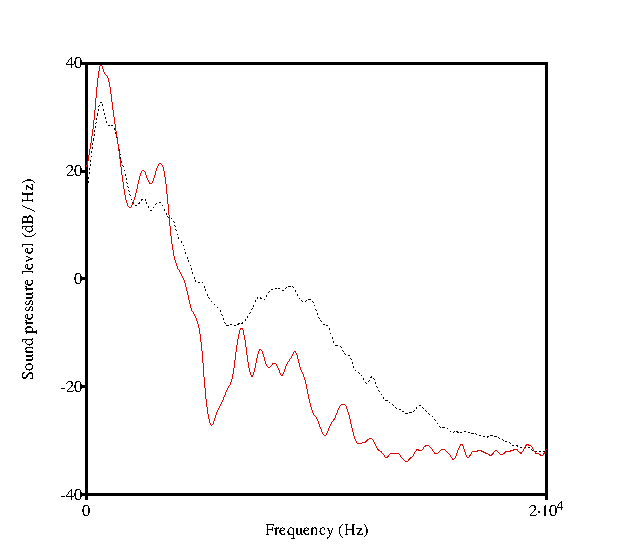
\includegraphics{figures/partialGlimpsing.eps}
	\caption[Partial glimpsing across frequencies at a particular time point]{Partial glimpsing across frequencies at a particular time point, illustrated by power spectrum of an [ɑ] vowel (solid red line) poking above the long-term average spectrum of the sentence from which the [ɑ] was extracted (dotted black line), at a signal to noise ratio of 0~dB. Both spectra have undergone cepstral smoothing with a 500 Hz bandwidth.\label{fig:PartialGlimpsing}}
	\end{centering}
\end{figure}

%\begin{figure}[htbp]
%	\begin{centering}
%	
\includegraphics{figures/xxx.eps}
%	\caption[Partial glimpsing over time in a particular frequency band]{Partial glimpsing in a particular frequency band over time, illustrated by the intensity of the waveform (solid red line) poking above the intensity of a speech-shaped noise masker (dotted black line).\label{fig:foo}}
%	\end{centering}
%\end{figure}

The main lesson to draw from glimpsing research is that energetic masking can vary along both temporal and spectral dimensions, just as the information contained in speech cues varies in its spectrotemporal distribution (compare brief broadband transients as cues for release bursts to slower-changing formant frequency patterns as cues to vowel quality, for example).  The fact that a single speech sound may have multiple non-simultaneous cues, combined with variation in the \term{robustness} and \term{precision} of those cues adds another layer of complexity to the picture.\footnotemark{}  Thus for a particular instance of speech masking it is difficult to quantify how much masking has occurred in terms of the \emph{information} recoverable.  Rather, measures of masking are often expressed in terms of the change in masker intensity (in dB) necessary to offset the difference in listener performance between two experimental conditions in a speech perception task.

\footnotetext{Here use \term{robust} to describe a cue that is maximally perceptible under a range of listening conditions (\ie, resistant to environmental masking), and \term{precise} to mean a cue that is maximally perceptually distinct from cues for other speech sounds in a given language (cf. definitions in \citealp{Wright2001, Wright2004b}, \citealp{Benki2003}, and \citealp[72 ff.]{HenkeEtAl2012}).  As one example, consider that an English [t] may be distinguished by the spectrum of its release transient, the relative duration of voice onset time (\ac{vot}), the direction of formant transition movement relative to the following vowel, and to some extent even the \emph{absence} of formant transitions due to the devoicing of the vowel during aspiration.  All of these cues vary in their precision and robustness, and in the competing English speech sounds that they help distinguish [t] from.}
% “A robust encoding involves cue redundancy, resistance of cues to environmental masking, the ability of cues to survive momentary distractions on the part of the listener, and the auditory impact of cues.” \citep{Wright2001}
% “Robustness of encoding can be defined along several dimensions: redundancy of cues, the auditory impact of cues, the perceptual distance between cues, and the resistance of cues to environmental masking.” \citep{Wright2004b}  
% “Following Wright (1996, 2004) and Benkí (2003), we define robustness as the degree to which the presence of a segment, and that segment’s contrastive information, is likely to be apprehended by a listener under normal listening conditions.  We define precision as the degree to which the cue narrows the field of segmental contenders (\eg\ Miller and Niceley 1955; McClelland and Elman 1986; Benkí 2003)” \citep[72 ff.]{HenkeEtAl2012}.

The difficulty of pinning down degree of energetic masking is exacerbated by the way that energetic and informational masking covary in certain masker types.  For example, in competing speech tasks one can reduce glimpses (both the likelihood of their occurrence and their spectrotemporal extent) and thereby increase energetic masking by increasing the total number of background speech streams (\ie, by using a \term{multitalker babble masker}).  However, this creates a situation where the background speech streams “mask” one another in addition to masking the target stream, such that the background speech itself becomes harder to understand.  This has the effect of decreasing informational masking, presumably by decreasing competition for lexical processing resources at higher levels of the brain’s speech processing stream.  In other words, although most research using babble maskers shows that the degree of total masking increases as the number of competing speech streams increases \citep[\eg][]{Miller1947, BrungartEtAl2001}, this result seems to be a combination of energetic masking going up even as informational masking goes down, making it difficult to separate the relative contribution of each to the total masking that is observed.  Recent research supports this view: \citet{SimpsonCooke2005} report that total masking seems to plateau around 6–8 background talkers, and further increasing the number of talkers causes the masking to recede back to a lower level seen with stationary, frequency-shaped random noise.  %This finding can be understood as a consequence of the interaction between energetic and informational masking just described: as the number of background talkers increases, the spectrotemporal glimpses tend to decrease (increasing energetic masking), while the informational content of any individual masker voice becomes increasingly obscured by competing background talkers (decreasing informational masking).  
This can be understood as a decrease in spectrotemporal variation in the masker stream due to an increase in number of background talkers (as background talkers fill in the gaps between one another’s words), such that the babble masker more and more closely approximates a random noise masker with spectral shape matching the long-term average spectrum of speech \citep{SimpsonCooke2005}.
%Put another way, as the number of talkers continues to increase, spectrotemporal variation decreases (as background talkers fill in the gaps between one another’s words) and the babble masker more and more closely approximates a random noise masker with spectral shape matching the long-term average spectrum of speech \citep{SimpsonCooke2005}.

To summarize, research on glimpsing shows us that not all forms of energetic masking are equal, and in a typical speech-in-noise task much depends on the frequency and timing of spectrotemporal glimpses with regard to the spectrotemporal location of target speech cues.  This is due to the fact that listeners use whatever information is available to make their best guess as to the content of the target speech, drawing on their perceptual experience at many levels of representation to “fill in the details” as the signals travel up through the language-processing pathways of their brains.  The next two sections discuss how masker signals can interfere at those higher levels to cause informational masking, either by sharing some crucial features with the target signal (target-masker similarity), or by virtue of frequent changes in some relevant aspect of the target-masker relationship (yielding low predictability from trial to trial, \ie, listener uncertainty).

\subsection{Target-masker similarity\label{sec:Similarity}}
Target-masker similarity can occur along a variety of dimensions, from fine-grained comparisons of spectral similarity (\eg, tone complexes masked by similar tone complexes, as in \citealt{LeeRichards2011}) to more abstract properties of the signals, such as the lexical token frequency of words.  This section reviews various dimensions of target-masker similarity that have been shown to affect masking.

One well-studied property of target-masker similarity is the perceived spatial origin of the competing streams.  Fundamentally, the localization of sound sources is perceived on the basis of interaural differences in timing and level of incoming sounds (\citealp[\eg][]{Hirsh1950, Kock1950}; see \citealp{Darwin2008} for review).  Numerous studies have shown a release from masking due to (actual or simulated) spatial separation between the target and masker streams \citep[\eg][]{CarhartEtAl1968, FreymanEtAl1999, BrungartSimpson2002, FreymanEtAl2004, GallunEtAl2005, KiddEtAl2005a, JohnstoneLitovsky2006}; the neural circuits underlying this ability are thought to reside in the lateral superior olive in the auditory brainstem \citep{ParkEtAl2004, TollinYin2005}.  Strictly speaking, interaural timing and level differences are not properties of the target and masker signals \perse, but of their relationship to the auditory system of a binaural listener.  Nonetheless, spatial origin of the signals is often treated as one of the dimensions along which target-masker similarity increases masking.   % Foreknowledge of a target talker’s spatial location can also help \citep{KitterickEtAl2010}.

Similarity between the voices in the target and masker streams is also predictive of masking: perception of the target stream is most difficult when the voices in the target and masker streams belong to the same person, moderately difficult when the voices belong to same-gendered talkers, and least difficult when the target and masker voices belong to a gender-mismatched pair \citet{Brungart2001}.  It is unknown what properties of the talkers’ voices underlie this phenomenon, though it has been speculated that both low-level spectral discrimination and auditory attention may be at play \citep{HelferFreyman2008}.

Several studies have shown that the dialect, accent, or language of the target and masker streams affects masking.  For example, native English listeners perform better on English target speech when the masker speech is Spanish \citep{GarciaLecumberriCooke2006}, Dutch \citep{BrouwerEtAl2012}, or Modern Standard Chinese \citep{VanEngenBradlow2007} rather than English.  Analogous experiments by \citet{RhebergenEtAl2005} showed similar effects for Dutch listeners exposed to Dutch target speech with either Dutch or Swedish maskers.  The release from masking seen with mismatched target and masker languages is smaller or absent in cases where the masker language is comprehensible to the listener, even if it’s not their native language \citep{GarciaLecumberriCooke2006, VanEngen2010, BrouwerEtAl2012}.  Likewise, for English target speech and native English-speaking listeners, masking is higher for native English competing speech than for foreign-accented English competing speech \citep{CalandruccioEtAl2010}.\footnotemark{}

\footnotetext{Corollary experiments confirmed that the difference was due to variation in the intelligibility of the background talker, not spectrotemporal differences between the masker streams \citep{CalandruccioEtAl2010}.}

Although findings regarding dialect, accent, or language mismatch between target and masker are sometimes attributed to target-masker similarity, they are perhaps better understood in terms of the availability, accessibility or perceptibility of the information in the masker stream \citep{VanEngenBradlow2007, CalandruccioEtAl2010, BrouwerEtAl2012}.  In other words, it is not necessarily the similarity of the target and masker languages or dialects that matters, but rather the degree to which elements of the masker stream are recognizable by the listener, on the assumption that such recognition causes competition between masker and target at later stages of auditory processing.  Support for this view comes from the finding that informational masking (indexed by reaction time) correlates with the lexical token frequency of the words in the masker speech \citep{BoulengerEtAl2010}.  Relatedly, \citet{BrouwerEtAl2012} showed that semantically anomalous English sentences provide less masking than semantically coherent ones, but no similar effect was found for English target speech masked by semantically well-formed and anomalous Dutch speech.  
%Moreover, the phenomenon of lexical popout presumably becomes less likely as the number of competing speech streams increases, so if differences between maskers of differing language, intelligibility, or semantic content are found with high numbers of background talkers, some other explanation must be proposed.

Taken together, these findings support the view that some cases of informational masking can be explained by \term{lexical pop-out} of specific words in the masker speech.  According to such an explanation, comprehensible background speech can compete with target perception relatively late in the auditory processing stream (\ie, at the point at which lexemes are recognized or accessed).  In contrast (so the explanation goes), incomprehensible background speech (such as foreign-language babble) is unlikely to trigger lexical competition, except by dint of accidental similarity to native words (a very low probability occurrence).  Experiments comparing normal to time-reversed masker speech also provide support for the lexical pop-out explanation of informational masking, since \ac{srt}s are generally higher with forward (comprehensible) speech than with reversed (incomprehensible) speech.\footnotemark{}  These studies also suggest that a listener’s past experience (in the form of word frequency) and expectations (in the form of contextual probabilities of words) both play an important role in the formation of the speech percept.

\footnotetext{See, \eg, \citet{HoenEtAl2007}, though cf. \citealt{RhebergenEtAl2005} for a review of issues related to energetic forward masking in time-reversed speech.}

This reasoning can be extended to the findings of \citeauthor{CalandruccioEtAl2010}\ showing that high intelligibility (native) speech masks better than low intelligibility (foreign-accented) speech, on the assumption that words are high-intelligibility precisely because they more readily trigger lexical activation (due to, \eg, greater cue redundancy).  The findings of \citeauthor{BrouwerEtAl2012}\ (showing weaker masking from babble comprising semantically anomalous sentences) might also be explained by appeal to lexical pop-out, though the explanation is somewhat more tenuous: a lack of coherent semantic relationships between early and late words leads to a reduction of semantic priming effects, thus decreasing the likelihood of lexical activations due to words in the masker stream, thereby reducing lexical competition from the masker stream.  

In sum, there seems to be value in reclassifying most reported cases of target-masker linguistic “similarity” as cases of lexical interference from the masker speech stream.\footnotemark{}  Of course, languages may be similar along many dimensions, both above and below the lexical level (\eg, typical grammatical or intonational patterns, the presence or absence of particular speech sounds or sequences, \etc).  The effect of such similarities in speech-on-speech masking situations is thusfar not well studied.  Nevertheless, target-masker similarity does seem an important consideration with regard to talker voices and spatial location.  Finally, the notion of listener uncertainty may offer additional insights into many of the findings discussed above; this topic is addressed in the following section.
  
\footnotetext{Cf. the distinction in \citet{Watson2005} between target-masker \term{structural similarity} and target-masker \term{representational similarity}.}
 
\subsection{Masking and listener uncertainty\label{sec:uncertainty}}
In laboratory settings, another apparent source of informational masking is the trial-to-trial regularity of the target and masker stimuli.  Experiments with pure-tone targets and pure-tone complexes as maskers have shown significant release from masking when the masker is held constant for the two intervals of each trial, even when the masker still varies spectrotemporally between trials \citep{NeffGreen1987, NeffCallahan1988}.  Similar results (again using tone complexes) have been obtained for masker spatial location \citep{FanEtAl2008} and temporal location \citep{BoninoLeibold2008}.  Related results show that target uncertainty is also relevant: the presence of notched-noise maskers or off-frequency tone complex maskers induces a considerable cost (quantified via target detection threshold) when listeners must attend to two different frequency regions in a tone-perception experiment \citep{KiddEtAl2008}.  Additionally, stimulus uncertainty has been shown to interact with target-masker similarity, such that masking under conditions of stimulus uncertainty is stronger when target and masker are more similar \citep{DurlachEtAl2003b}.  Such results suggest that listener uncertainty (or conversely, stimulus predictability) is important to a full account of informational masking.

The advantage seen in situations of masker predictability is presumably attributable to a listener’s ability to adapt to, suppress, or \term{tune out} information from maskers that are constant from trial to trial.  Early studies of listener uncertainty using speech stimuli showed higher word-recognition scores for blockwise presentation of a single talker compared to mixed-talker blocks \citep{SommersEtAl1994}, suggesting that listeners can also accommodate (or \term{tune in}) to a particular voice when target talker identity is predictable (a finding replicated in \citealt{BrungartSimpson2004} and \citealt{EricsonEtAl2004}; cf. also the discussion of training studies in Section~\ref{sec:Training}).  Similar results are seen when holding fixed other dimensions of the stimuli.  For example, in a closed-set response task using the \ac{crm} corpus, holding fixed the semantic content of the masker stream leads to a release from masking even when the voice speaking the masker phrase changes trial-to-trial \citep{BrungartSimpson2004}.  Other studies have shown that uncertainty about the spatial location of the target speech (in the presence of competing, spatially distinct speech streams) results in dramatically lower target perception success than cases where the location of the target speech is known \citep{EricsonEtAl2004, KiddEtAl2005a}.  However, the generalizability of findings based on small-vocabulary response sets is uncertain: a study using nonsense sentences as targets and maskers found little to no effect of stimulus variation (and hence listener uncertainty) in \ac{snr}, talker identity in the masking stream, or masker content \citep{FreymanEtAl2007}.

In general, experiments exploring stimulus uncertainty using speech maskers have been less common than studies using non-speech stimuli, presumably due to the difficulty of controlling and quantifying the spectrotemporal similarity of speech maskers (as can be done fairly readily with tone complexes).  Despite this relative lack of research, stimulus uncertainty may turn out to play a role in explaining previous findings thought to be related to target-masker similarity.  For example, increased masking from native- \vs\ foreign-language babble maskers \citep[\eg][]{RhebergenEtAl2005, GarciaLecumberriCooke2006, VanEngenBradlow2007, BrouwerEtAl2012} might be explained as a difference in stimulus uncertainty: in the foreign-language babble, the accessible semantic content is constant and predictable (\ie, null) whereas the native-language babble has varying semantic content with regard to lexical activation (in that the identity and timing of words that pop out of the babble can vary from trial to trial).  Further research is needed to disentangle the roles of similarity and uncertainty under such circumstances.  %Similarly, the weaker masking due to semantically anomalous native-language babble \citep{BrouwerEtAl2012} could be construed as a stimulus uncertainty problem, 

\subsection{Summary of masking research}
The studies reviewed above show various ways in which speech perception degrades under adverse conditions.  The picture that emerges is one in which listeners use whatever information is available to aid in the perceptual task, relying on information at many levels in the speech processing stream.  One final study bears mentioning here, which shows that listeners adapt their listening strategy to the particular type of adversity they are confronted with.  \citet{MattysEtAl2009} show that severe signal degradation (\ie, energetic masking) tends to promote reliance on acoustic speech cues that escape the noise, and reduce reliance on higher level lexico-semantic cues.  In contrast, situations involving depleted cognitive resources or divided attention (\ie, informational masking) tend to increase reliance on lexico-semantic cues.  Thus for any investigation of speech perception under adverse conditions, one must always be cognizant of the different types of information available to the listener (either in the signal or as part of her linguistic experience and expectations), and consider which types of information are likely to be compromised by a given masker type. 

% % % % % % % % % 
% % % % % % % % % 
% PROGRESS MARKER 
% % % % % % % % % 
% % % % % % % % % 

\section{Intelligibility}
This section first reviews past findings on intelligibility related to four commonly measured acoustic dimensions of speech: vowel formant frequencies, duration, intensity, and pitch.  %This is followed by a discussion of segmental features and cues, particularly as related to the phenomena of clear speech, speech reduction, and Lombard effects.  Next, these dimensions of speech are related to talker characteristics such as gender, dialect, sociolect, and foreign accent.  The section concludes with a brief discussion of the role of the listener in intelligibility, focusing on peripheral hearing loss and age-related cognitive decline.%, with brief mention of specific language impairment (SLI) and central auditory processing disorder (CAPD).
This is followed by a discussion of speech style, focusing on clear speech and Lombard effects.  Finally, listener contributions to speech perception are reviewed, focusing on language proficiency, hearing loss, cognitive factors, and attention.

\subsection{Intelligibility and vowel formant frequencies\label{sec:IntelVowel}}
Much research supports the idea that intelligibility is linked to properties of the F2×F1 vowel space \citep[\eg][]{BondMoore1994, BradlowEtAl1996, HazanMarkham2004, Neel2008, McCloyEtAl2013}, though precisely which properties of the vowel space correlate with intelligibility is still an unresolved question.  From both word-identification and sentence-comprehension experiments, there seems to be consistent evidence for the overall size of the vowel space as a predictor of intelligibility, though different studies have used different metrics of vowel space size.  Size-related measures reported to positively correlate with intelligibility include F1 range \citep{BradlowEtAl1996}, F2 range \citep{HazanMarkham2004}, mean distance of vowel tokens from the center of the vowel space \citep{BradlowEtAl1996, McCloyEtAl2013}, area of polygon formed by vowel means (\citealt{BradlowEtAl1996}: /i~o~a/; \citealt{Neel2008}: /i~æ~ɑ~u/;  \citealt{McCloyEtAl2012}: /i~ɪ~e~ɛ~æ~a~ɔ~o~ʊ~u/), and area of the convex hull encompassing all vowel tokens \citep{McCloyEtAl2013}.

The area of the convex hull is arguably the most appropriate metric of vowel space expansion, since measures like F1 and F2 range may be more sensitive to dialectal variation, and values for mean distance from center will vary dramatically depending on which vowels are included in the analysis (see \citealt{McCloyEtAl2013} for discussion).  More research is needed to determine which of these metrics is most stable across languages and talker groups, and which most reliably indexes differences in intelligibility.

Another important aspect of the F2×F1 vowel space is the degree of vowel phoneme overlap or \term{phonemic crowding}.  Phonemic crowding can be indexed by the total repulsive force of the vowel system \citep[see][]{McCloyEtAl2013}.  Mean vowel cluster size indexes the within-category variability of the vowel phonemes, which is related to (and likely to co-vary with) phonemic crowding \citep{McCloyEtAl2013}.  

% TODO: say something about vowel reduction here.

\subsection[Intelligibility and duration]{Intelligibility and duration: Speech rate and speech rhythm\label{sec:IntelDur}}
One of the earliest studies of the relation between intelligibility and speech rate was performed by \citet{Tolhurst1957a}, who found a significant effect for duration among three speech styles (prolonged, normal, and staccato) in an analysis of variance test.  In more recent studies, evidence has been mixed as to whether speech rate is predictive of intelligibility.  For example, \citet{SommersEtAl1994} found a significant effect of variation in speech rate on intelligibility, suggesting that speech rate is one of the factors relevant to masking due to listener uncertainty.  In contrast, \citet{BradlowEtAl1996} found no correlation between mean sentence duration and intelligibility, and \citet{KrauseBraida2002} found that the intelligibility difference between clear and conversational speech is apparently independent of speaking rate.  Examining word durations, \citet{BondMoore1994} found differences in isolated word durations between two talkers of varying intelligibility, but not in words in sentential context.  Finally, in a modern study echoing \citet{Tolhurst1957a}, \citet{MayoEtAl2012} examined plain, infant-directed, computer-directed, foreigner-directed, and shouted speech, finding a correlation between sentence duration and word error rate across speech styles, as well as significant segment length differences across speech styles for stops, fricatives, nasals, vowels, and diphthongs (but not affricates, liquids or glides).  Their findings suggest that “much of the prosody-related intelligibility gain comes from durational increases” \citep{MayoEtAl2012}.

To the extent that duration co-varies with other dimensions of linguistic variability (\eg, segmental reduction), it is unsurprising that duration can be predictive of speech intelligibility.  However, it remains unclear whether measurements of duration reflect a genuine percept in the speech perception process, or are merely a convenient surrogate for other, harder-to-measure factors like segmental reduction or the occurrence of spectrotemporal glimpsing.

There is also some evidence that patterns of duration (\ie, rhythm) can contribute to speech intelligibility.  The proper description and classification of linguistic rhythm has been a long-standing debate in the field, and a thorough rehashing of those issues is beyond our purposes here.\footnotemark{}  Nonetheless, two studies bear reporting here for their relation to intelligibility.  First, with regard to duration in foreign-accented speech, \citet{QueneVanDelft2010} found that the speech reception thresholds (\ac{srt}) of high-intelligibility non-native Dutch sentences were improved when the sentences were resynthesized to match the durational patterns of a native Dutch speaker, while the \ac{srt} of native Dutch speech was degraded when the native sentence was resynthesized to have the durational patterns of non-native speech.  Second, in a 2×2 design investigating native duration patterns and syllable-isochronous duration patterns where all stimuli had been monotonized, it was found that target speech perception was above chance only when the target had native-like duration patterns and the competing speech had syllable-isochronous duration patterns \citep{CushingDellwo2010}.  In other words, subjects performed near chance when either the masker had native-like durations, or the target had syllable-isochronous durations.  
\footnotetext{A succinct summary of the issues and evidence regarding the classification of linguistic rhythm can be found in \citep{Ramus2002}.}

Both of those studies suggest an intelligibility benefit for sentence-length stimuli with native-like durational patterns.  The relationship between rhythmic variations (\eg, between native-like and non-native-like rhythms) and summary measures of duration (\eg, mean sentence length) is not well understood (cf. \citealt{Ramus2002}).  One recent study looking at differences in temporal structure between conversational and clear speech primarily found differences in occurrences of vowel and consonant reduction and deletion, leading to differences in the number of prosodic phrases, but an overall consistency across speech styles in the ratio of consonantal to vocalic stretches and the variability of each \citep{SmiljanicBradlow2008}.  In other words, consonants and vowels were both subject to durational reduction in conversational style (in roughly equal measure), and the variability in consonant and vowel duration remained constant across speaking styles (relative to the overall speech rate).

Of course, there is more to rhythm than simply duration patterns, and neither \citet{QueneVanDelft2010} nor \citet{CushingDellwo2010} accounted for differences in intensity patterns between the native and non-native conditions (though both did equate the mean intensities of all stimuli).  A discussion of the relation between intensity and intelligibility follows in Section~\ref{sec:IntelIntens}; unfortunately there will be little to say about rhythmic patterns of intensity as related to speech intelligibility, as such research is still in its infancy (though see \citealt{TilsenJohnson2008} for a recent inroad into quantifying speech rhythm through Fourier analysis).

% see also:
% \citep{Klatt1976, WightmanEtAl1992}: linguistic use of duration in general
% \citep{RamusEtAl1999}: acoustic correlates of rhythm
% \citep{RaoSmiljanic2011}: age, clear speech & rhythm in English and Croatian
% \citep{LiuZeng2006}: time-compression and silence addition to change speech rate of clear and conversational speech.
% \citep{SundaraScutellaro2011}: rhythmic distance affects bilingual infants’ acquisition.
% \citep{DellwoHagmann2011}: the processes that underly the perception of duration seem to be sensitive to linguistic structure; contrastive length affects duration percepts.

\subsection[Intelligibility and intensity]{Intelligibility and intensity: Audibility and \ac{snr}\label{sec:IntelIntens}}
When considering the relationship between the intensity of speech and its intelligibility, the most obvious consideration is whether the speech is loud enough to be above the listener’s auditory thresholds in the relevant frequency regions.  In other words, for speech to be intelligible it must be audible.  In real-world settings this is affected not only by the source power of the talker’s speech, but also by the distance between talker and listener, their relative head orientations, the presence of background noise, and any irregularities in auditory thresholds of the listener (\ie, hearing loss or congenital deficit).

In contrast, laboratory settings offer controlled signal levels, minimal background noise, and minimal or no effect of head orientation due to the use of headphones (or fixed head position with free-field sound sources).  Irregularities in auditory thresholds can also be accounted for by audiometric testing of listeners.  Thus in the laboratory audibility is well within the experimenter’s control, and the most important audibility consideration becomes the intensity contour of the target signal itself, especially in relation to different masking signals.% and \ac{rms} normalization.

In all speech stimuli there is considerable variation in intensity across the span of the stimulus.  Some of this variation is due to inherent differences in intensity of different speech sounds.  For example, in general the vowel [ɑ] is louder than [i] \citep{Ladefoged1967}, [f] is quieter than [s] \citep{sowl}, and vowels are usually much louder than consonants \citep{HoriiEtAl1971}.  In sentence-length or longer stimuli, there is also variation in the mean intensity of each word.  This variation is not random, but rather is determined by linguistic properties of the speech, in particular lexical stress and phrasal accent \citep{Fry1955, SluijterVanHeuven1996, PlagEtAl2011}.  There is also a cross-linguistic tendency for words at the ends of utterances to be quieter than words near the start of the utterance \citep{StrikBoves1995, TrouvainEtAl1998}.  For speech presented in background noise, this can lead to differences in \ac{snr} across the span of the utterance, and increase or decrease the probability of glimpsing a particular word depending on its position or role in the sentence (cf. Section~\ref{par:Glimpsing}).  

One approach to the variability of intensity across utterances is to use an amplitude-modulated masker that tracks the amplitude envelope of the target speech, thereby keeping \ac{snr} effectively constant at a fairly short temporal scale (instead of calculating \ac{snr} at the whole-stimulus level, as is more typical).  However, some cues to the identity of speech sounds are preserved in the amplitude envelope, making envelope-tracking maskers less effective than stationary maskers in some cases (\citealp{HoriiEtAl1971, VanTasellEtAl1987, BashfordEtAl1996}; see \citealp{Wright2004b} for review).

More fundamentally, there are aspects of suprathreshold hearing and speech perception that are level-dependent.  For example, \citet{DubnoEtAl2012} report that speech envelope cues (\eg, manner cues that help distinguish fricatives from stops) are most readily perceived at around 60 {dB} \ac{spl}, with performance declining at both lower and higher intensities.  The decline in speech reception at high intensities is usually termed \term{rollover}, and has been shown to be somewhat frequency-dependent: rollover is stronger for high-frequency and broadband sounds than for low-frequency sounds, in both normal-hearing and hearing-impaired listeners \citep{SummersCord2007}.  However, the level at which rollover begins varies between normal-hearing and hearing-impaired populations \citep{SummersCord2007}, and in general listeners with hearing impairment gain less advantage from supra-threshold changes in signal level than do normal hearing listeners \citep{SummersMolis2004}.

Aside from considerations of audibility and glimpsing, there seems to be little relationship between intensity and intelligibility as long as intensity variations are relatively modest.  The findings of \citet{BondMoore1994} are typical: they report no significant differences in intensity in the speech of their three talkers (even though the recordings were not \ac{rms} normalized), but the talkers varied considerably in intelligibility nonetheless.  Indeed, numerous studies using \ac{rms}-normalized stimuli show variation in talker intelligibility despite equivalent intensities of stimuli \citep[is one example]{McCloyEtAl2013}.

\subsection[Intelligibility and pitch]{Intelligibility and pitch: Gender and voice quality\label{sec:IntelPitch}}
A number of studies have looked for a significant relationship between intelligibility and the fundamental frequency (\fo) of speech.  Typically, what is found is that static measures of pitch such as mean \fo{} do not correlate well with speech intelligibility \citep[\eg,][]{PichenyEtAl1986, BradlowEtAl1996, HazanMarkham2004, LuCooke2009}, suggesting that gender differences in intelligibility are merely {\em indexed} by differences in mean pitch, rather than {\em caused} by them \citep[cf. discussion in][]{BradlowEtAl1996}.  In contrast, measures that reflect a talker’s dynamic use of pitch do seem to be relevant to intelligibility.  For example, both \citet{BradlowEtAl1996} and \citet{McCloyEtAl2013} report a positive correlation between a talker’s \fo{} range and intelligibility, and \citeauthor{McCloyEtAl2013}\ also report a significant effect for rate of change of \fo{} (\aka, \term{pitch dynamicity}, cf. \citealt{GauthierEtAl2007b, GauthierEtAl2007a, GauthierEtAl2009}). %TODO: add something about Motherese here?  Sharon mentioned it.

Studies of intelligibility with manipulated \fo{} contours also show intelligibility effects.  \citet{BinnsCulling2007} report a significant increase in \ac{srt} in an English competing speech task when the \fo{} contour of target speech is flattened or inverted, but no effect when the masker speech is similarly manipulated.  \citet{WatsonSchlauch2008} report similar results for speech with flattened \fo{} in white noise.  Unsurprisingly, flattening pitch contours also impacts intelligibility in lexical tone languages like Modern Standard Chinese \citep{PatelEtAl2010}.

% see also:
% BraunEtAl2011: unfamiliar intonation slows down processing: compared unattested "sinewave" intonation to normal Dutch intonation in three different reaction time tasks.
% Holm2007: L2 Norwegian by English/Dutch L1 speakers is more intelligibile if resynthesized to have native-like intonation (though note pitch is semi-lexical in norwegian).

Another issue related to fundamental frequency concerns voice quality or phonation.  Laryngealization or \term{creaky voicing} is common as a prosodic marker \citep{Lehiste1979, Kreiman1982, DilleyEtAl1996}, and is associated with a drop in both \fo{} and intensity \citep{GordonLadefoged2001}.  The drop in intensity makes creaky-voiced words particularly susceptible to masking due to elevated word-level \ac{snr}, particularly with stationary noise maskers.  %This is particularly common in utterance-final position due to pitch declination in common utterance types (\eg, neutral declarative prosody in American English).

Pitch and voice quality can also be exploited for sociolinguistic purposes (\ie, to index gender or sexual orientation; see \citealt[\intal]{McconnellGinet1978, Gaudio1994, Podesva2011}), and the linguistic uses of pitch are not necessarily consistent across languages \citep{MajewskiEtAl1972, Todaka1993, Yuasa2008, KeatingKuo2012}, dialects \citep{GrabePost2002, ClopperSmiljanic2011}, or sociolects \citep{McLemore1991, Britain2008}.  %Within American English, pitch accent, boundary tone, and pause distribution also varies with regional dialect and gender \citep{ClopperSmiljanic2011}.  
% For example, \citeauthor{Todaka1993} examined the speech of bilingual speakers of English and Japanese (both L1 English speakers whose L2 was Japanese, and \vv), and found that mean pitch was significantly higher for all speakers (both male and female) when speaking Japanese than when speaking English \citep[126–130]{Todaka1993}.\footnotemark{}  Other studies include \citet{MajewskiEtAl1972} comparing American English to Polish, and \citet{KeatingKuo2012} comparing American English to Modern Standard Chinese.
Moreover, style-based changes in pitch are often accompanied by changes in other dimensions that are relevant to intelligibility (\viz\ intensity, duration, and vowel formant frequencies, cf. Section~\ref{sec:SpeechStyle}).  This makes correlations among intelligibility and the acoustic dimensions of speech difficult to disentangle, and any individual finding should be interpreted cautiously.  It also underscores the need for studies of intelligibility that vary these acoustic dimensions independently (a feat only possible with resynthesized or fully synthetic speech).

%\subsection{Other segmental cues\label{sec:SegCues}}
% Discussion of non-vowel reduction.  presence of stop release bursts \citep{PichenyEtAl1986, LiLoizou2008}.  Intelligibility in various simulated environments w/r/t vowel ID, consonant contrasts in voicing, continuance, place \citep{CoxEtAl1987}.  Relate to redundancy, smooth signal hypothesis, etc.

\subsection[Intelligibility and speech styles]{Intelligibility and speech styles: Clear, reduced, and Lombard speech\label{sec:SpeechStyle}}
It is well known that talkers have some control over the intelligibility of their speech, in that a single talker can adopt different speaking styles that vary in intelligibility.  Early work by \citeauthor{Tolhurst1957a} on intelligibility and speech styles was discussed in Section~\ref{sec:IntelDur} with regard to speaking rate \citep{Tolhurst1957a}; related studies examined the effect of instructions to talkers to speak clearly \citep{Tolhurst1954, Tolhurst1955}.  More recently, research into the intelligibility of speech styles has focused on \term{clear speech} — speech directed toward listeners who are hard of hearing and produced with intent to aid comprehension — a line of research pioneered by Durlach, Braida and colleagues \citep[\eg][]{PichenyEtAl1985, PichenyEtAl1986, PichenyEtAl1989, UchanskiEtAl1996, KrauseBraida2004}.  These and related studies show intelligibility improvements in the range of 10–20\% over conversational speech.

The acoustic differences between clear and conversational speech span a range of acoustic parameters discussed in Sections~\ref{sec:IntelVowel}–\ref{sec:IntelPitch}, including changes in vowel formant frequencies, speech rate (due to both longer words and more pauses in clear speech), intonation patterns, and segmental reduction or deletion \citep[see][\intal]{PichenyEtAl1986, LiLoizou2008, SmiljanicBradlow2008, HazanBaker2011}.  However, precise characterization of each parameter’s contribution to intelligibility is elusive, due at least in part to the processing artifacts that arise in speech resynthesis, which is necessary to manipulate these parameters independently \citep[cf. discussions in][]{PichenyEtAl1989, UchanskiEtAl1996, LiuZeng2006, KrauseBraida2009}.

A related line of research involves the changes to speech produced in the presence of background noise (often called \term{Lombard speech} after Etienne Lombard, who first characterized the phenomenon).  Lombard speech has been shown to involve changes in intensity, pitch, formant frequencies, and duration \citep{LaneTranel1971, SummersEtAl1988}, though the changes are less pronounced than with read clear speech \citep{HazanBaker2011}.  Interestingly, talkers’ adjustments seem to be sensitive to the content of their speech: at high noise levels, the \fo{} and duration of words bearing a high informational load will be preferentially modified \citep{PatelSchell2008}.  Speech alterations due to the Lombard effect seem to be automatic, subconscious, and difficult to suppress \citep{PickEtAl1989}, and quite variable from talker to talker \citep{Junqua1993}.  Nonetheless, Lombard speech has been shown to be more intelligible than speech produced in quiet \citep{DreherONeill1957, SummersEtAl1988}, though again, the contributions to intelligibility changes due to various acoustic dimensions of speech remains unclear.

% see also:
% \citep{SmiljanicBradlow2011}: Clear speech benefits both native and non-native talkers and listeners.
% \citep{LuCooke2008, LuCooke2009, CookeLu2010, VillegasCooke2012} Intelligibility of speech produced in noise; mostly looking at pitch and spectral tilt.

\subsection{Intelligibility and linguistic content}
To a first approximation, Sections~\ref{sec:IntelVowel}–\ref{sec:SpeechStyle} deal with correlates of speech intelligibility at the level of the acoustic signal (intensity, duration, pitch) and at the phonetic\slsh phonological level (vowel space characteristics).  This section discusses relationships between speech intelligibility and lexico-semantic aspects of the speech signal.

One aspect of a word that can influence its intelligibility in noise is how frequent or common the word is.  Numerous studies have shown a perceptual advantage for high-frequency words in lexical decision tasks (word\slsh non-word judgments) in both reaction time and accuracy, as well as higher intelligibility in speech-in-noise tasks \citep[\eg,][]{Howes1957, Savin1963, VitevitchLuce1998, DirksEtAl2001, TakayanagiEtAl2002, VitevitchRodriguez2005}.  In competing speech tasks with sentence-length stimuli, high-frequency words are also more likely than low-frequency words to pop out of the background and cause distraction (\ie, retard reaction time or cause a misperception of a target word for a background competitor; \citealt{BoulengerEtAl2010}).

Another important consideration is the \term{neighborhood density} of the word.  Neighborhood density is usually defined as the number of other words in the lexicon that differ by only one phoneme by substitution, addition, or deletion \citep{LucePisoni1998}.  Words from sparse lexical neighborhoods are typically more readily perceived than words from dense lexical neighborhoods \exclude{, again both in terms of reaction time and accuracy in lexical decision tasks, and in terms of intelligibility in speech-in-noise tasks} \citep{VitevitchLuce1998, ZieglerEtAl2003}, although this does not seem to be universally true of all languages \citep{VitevitchRodriguez2005}.  A third consideration is \term{neighborhood frequency}, or the mean lexical frequency of all the phonological neighbors of a word; a high neighborhood frequency generally impedes word perception \citep{LucePisoni1998}.  
% although occasionally neigborhoods are constructed on the basis of syllables rather than phonemes \citep{xxx}.

% \citep{VitevitchLuce1998}: Phonotactics matters, as seen with nonwords (Prelexical).  In real words, good phonotactics goes along with dense neighborhoods, so the two foces compete.
% \citep{VitevitchRodriguez2005}: Spanish auditory word recognition (word\slsh nonword): high frequency => faster; dense neighborhood => faster (unexpected); high frequency word + high frequency neigborhood => faster (unexpected)
% \citep{ZieglerEtAl2003}: French auditory word recognition (word\slsh nonword): phonological density => slower, more errors.  Orthographic density => faster, fewer errors.

Finally, the semantic context of words in sentences contributes to their intelligibility.  For example, \citet{LewisEtAl1988} showed that words that are predictable from context are harder to mask, in that they are recoverable (or at least guessable) at lower \ac{snr}s than the same words in low-context sentences.  At the same time, words that are predictable from context are typically articulated less distinctively, as though the talker were balancing their own articulatory effort with expectations that the listener is paying attention and can recover some words more easily than others \citep{Wright2004a}.

% see also:
% \citep{HoenEtAl2007}: “lexical masking occurs only when some words in the babble are detectable, i.e. for a low number of talkers, such as 4, and diminishes with more talkers.”
% \citep{BrouwerEtAl2012}: showed that semantically anomalous English sentences provide less masking than semantically coherent ones, but no similar effect was found for English targets masked by semantically well-formed and anomalous Dutch speech.
% \citep{CreelEtAl2008}: “lexical competition was attenuated by consistent talker differences between words that would otherwise be lexical competitors” (eye tracking)

\subsection{Listener contributions to intelligibility\label{sec:Listener}}
There are at least three aspects of the listener that are relevant to considerations of speech intelligibility: hearing impairment, cognitive capacity, and language proficiency.  A fourth factor, familiarity with the voice of the talker, will be discussed in detail in Section~\ref{sec:Fam}.  

A thorough characterization of the types and causes of hearing impairment is beyond the scope of this work.\footnotemark{}  However, for our purposes it suffices to state that most types of age-related hearing loss typically involve elevated detection thresholds (especially in frequencies above 4 kHz), and decreased frequency selectivity (\ie, broader auditory filter bandwidths) across all frequencies.  This increases the difficulty of the signal detection task that underlies auditory perception generally (making it hard to separate target from background), and also impairs perception of the spectral composition of sounds (which can make certain speech sounds more difficult to discriminate).  See \citet[117–119]{Moore2008} and references therein for more detailed discussions.

\footnotetext{See \citet[chap.\ 10]{Pickles2008} for overview, or \citet{SataloffSataloff2005} and \citet{GordonSalantEtAl2010} for detailed treatments.}

A variety of studies suggest that, like most perceptual tasks, speech perception becomes more difficult under increased cognitive load.  For example, \citet{FrancisNusbaum1996} performed a syllable recognition task with a simultaneous digit span recall task, and showed that reaction time slowed under high cognitive load when there was variability in speech rate of the stimuli.  \citeauthor{FrancisNusbaum1996} interpret this finding as evidence that speech perceptual tasks like talker- or rate-normalization are active rather than passive perceptual processes and induce a cognitive load.  

Recent research supports this view of speech perception as cognitive load: \citet{MattysEtAl2009} report that competing talker tasks increase reliance on lexico-semantic cues, whereas noise masking increases reliance on low-level acoustic cues.  The link between reliance on lexico-semantic cues and cognitive load comes from findings that older listeners (with diminished cognitive resources) benefit more from contextual (lexico-semantic) cues than do younger listeners \citep{PichoraFullerEtAl1995, SommersDanielson1999}.  % See also: FedermeierEtAl2002: ERP study of age and semantic context

A related consideration concerns auditory attention and the distribution of attentional resources.  In a divided listening task using the \ac{crm} corpus, \citet{BestEtAl2006} showed that listeners perform substantially worse when asked to report keywords from both of two simultaneous speech streams, especially when the two speech streams are widely separated spatially.  This latter finding is surprising given that spatial separation of target and masker streams {\em aids} the perceptual task when only one stream is the focus of attention, as does prior knowledge of the target’s spatial location (cf. \citealt{KiddEtAl2005a}, and discussion of spatial separation in Section~\ref{sec:Similarity}).  

Prior knowledge of how to direct attention also helps listeners overcome high cognitive load.  Knowledge of talker identity, spatial location, and timing improved \ac{srt} of target speech in a 26-talker listening task in which pairs of talkers began synchronously (with the 13 pairs staggered at regular intervals), but such knowledge was much less useful in a similar 13-talker task in which each talker had a unique temporal onset \citep{KitterickEtAl2010}.  In corollary experiments that slightly staggered the onsets of the target-masker pair (but not the distractor pairs), an advantage was seen only when the target onset fell on the regular rhythmic timing slot set up by the distractor pairs’ onsets, indicating that knowledge of when the target speech would begin allowed the listeners to benefit from the onset asynchrony between target and masker.

Distribution of perceptual processing resources can also come into play at a lower level than the willful apportionment of listener-directed (endogenous) attention.  In a series of binaural listening experiments, \citet{GallunEtAl2007} show that noise maskers presented contralaterally to the target signal can nonetheless mask the target in cases where the target and masker are spectrally similar and the task demands are high.  In other words, under high cognitive load, perceptual tasks that are normally possible become difficult to achieve (\eg, single-ear listening, or equivalently, suppression of cross-ear auditory object formation).  %These results suggest that some attentional or auditory processing resources may be recruited by the masker stream even when it is binaurally distinct from the target, clearly non-speech-like, and thus (one would expect) easy to tune out or ignore.  

% see also:
% \citet{CookeEtAl2008} foreign language cocktail party: divided attention.
% \citep{GallunEtAl2008}

As discussed in Section~\ref{sec:Similarity}, one of the factors that influences the degree of masking in a speech-on-speech task is the relationship between the native language of the listener and the language of the masker speech; masker speech that is comprehensible to the listener masks more strongly than foreign speech that the listener can’t understand.  This relationship applies to the target speech as well: a monolingual English speaker will obviously find Tamil target speech completely unintelligible, and as she begins to learn Tamil there will almost certainly be a period of first-language (\aka, L1) interference in her perception of Tamil speech sounds.  In one study demonstrating this, \citet{HazanSimpson2000} showed that in an English consonant identification task, the errors made by L1 Spanish speakers and L1 Japanese speakers differed in a way that was partly predictable from differences between English and the listeners’ native phonologies.  The pattern of errors was preserved even for stimuli with cue enhancement (selective amplification of formant transitions and release bursts), showing the robustness of L1 phonological interference.

In addition to interference from L1 segmental phonology, there are also subtle biases in cue weighting built into listener perceptual processes.  For example, \citeauthor{Zielinski2008} reports that native English speakers listening to non-native (L2) English speech preferentially rely on syllable stress patterns, and segmental cues within prominent syllables.  In other words, native listeners “[apply] native speech processing strategies to a non-native speech signal,” in a way that makes errors of stress placement particularly destructive to intelligibility \citep[80]{Zielinski2008}.

The degree and type of listener exposure to the language of the target speech is also an important consideration.  For example, \citet{PinetEtAl2011} showed that L1 French listeners with low-proficiency L2 English performed better when target speech was French-accented English than when target speech was native (Southern England) English, but the pattern was reversed for L1 French listeners with high English proficiency.  \citeauthor{PinetEtAl2011}\ attribute this finding to listener experience and exposure: the listeners with low-proficiency English had mostly been exposed to French-accented English in classroom settings, whereas the listeners with high-proficiency English had more broad exposure to the language.  Similar results have been reported for Spanish learners of English \citep{ImaiEtAl2005}, Chinese and Korean learners of English \citep{BentBradlow2003}, and speakers of many other languages.%  Presumably through familiarity with its lexicon, phonemic structure, and prosody...

% TODO: add to previous paragraph:
% \citep{FlocciaEtAl2006}: “lexical decision performance was slower and less accurate for unfamiliar dialects than familiar dialects” (French)

\section{Talker familiarity\label{sec:Fam}}
Section~\ref{sec:Listener} mentioned several studies in which familiarity with the language or dialect of the target speech conferred a perceptual advantage \citep[\eg,][]{BentBradlow2003, ImaiEtAl2005, PinetEtAl2011}.  A variety of studies have shown that familiarity with a talker’s voice is also advantageous.  Many such studies involve training listeners to reliably identify previously unknown talkers by voice alone.  Typical methodology involves a period of exposure to voices paired with names, followed by a training phase where listeners must supply the names but are given immediate feedback, and a final testing phase where listeners supply the names of talkers and no feedback is given.  The training studies discussed in Section~\ref{sec:Training} all use some variant of this procedure, but vary in the number of talkers to be identified, the type of training and\slsh or testing stimuli (words \vs\ sentences; native \vs\ foreign speech), the presence and type of masking noise in the training and\slsh or testing phase, and various other subtle differences (\eg, associating voices with pictures instead of names).  Section~\ref{sec:LongTerm} discusses two studies in which longer-term familiarity with a talker’s voice is investigated.

\subsection{Training studies\label{sec:Training}}
A foundational study establishing a familiarity advantage in speech perception was \citet{NygaardEtAl1994}, in which listeners trained for nine days to associate ten voices with ten common first names (five male, five female) based on single-word utterances.  On the tenth day, listeners correctly identified talkers based on new words not in the training set, showing that successful talker identification was not limited to the actual words used in the training phase.  More importantly, listeners were presented words in various levels of background noise, and were significantly better at word identification in noise when the word was spoken by a familiar talker.

Another important early finding is that the familiarity advantage does not readily generalize across stimulus types.  Listeners trained to identify talkers based on single words did not benefit from talker familiarity when tested on sentence-length stimuli in noise; likewise, listeners trained to identify talkers based on sentential stimuli did not benefit from talker familiarity when tested on single-word utterances \citep{NygaardPisoni1998, YonanSommers2000}.  A corollary finding of this study is that talker identification training progresses much faster when based on sentential stimuli than when based on single words (three training sessions \vs\ nine to achieve comparable levels of talker identification success).     

The finding that talker identification training does not generalize to different stimulus types has been repeated in a variety of ways.  \citet{LeviEtAl2011} show that training monolingual English listeners to discriminate (bilingual) talkers based on German words confers no advantage when the listeners are tested on English words.\footnotemark{}  \citet{VanEngen2012} reports similar results when the training is carried out in different kinds of background noise: if listeners are tested on speech with a babble masker, they perform better when they were trained with a babble masker (rather than speech-spectrum noise) and when the language of the babble masker matches the language of the masker they were trained with.

\footnotetext{In fact, just learning to correctly discriminate talkers is difficult if the training speech is not readily comprehensible to the listener, either because it is a foreign language \citep{PerrachioneWong2007} or because of a phonological deficit such as dyslexia \citep{PerrachioneEtAl2011}.}

%Talker familiarity also has implications for explicit memory: listeners more accurately identify a word as old (\ie, occurred before in the list) when it is repeated by the same talker and at the same speech rate \citep{BradlowEtAl1999}.  

Finally, there are age-related differences in the ability to identify talkers and the ability to benefit from familiarity.  In one study, young listeners (age 18–24) were near ceiling (98\%) on a four-talker identification task on both days of training, while older listeners (age 66–87) hovered around 75\%.  However, older listeners paradoxically showed a greater benefit for talker familiarity in a speech-in-noise perception test at the end of the training, suggesting that older listeners were benefiting from implicit learning or exposure even if they could not make use of it in a talker identification task \citep{YonanSommers2000}.  A second experiment confirmed this: old and young listeners who were merely exposed to talkers in an orthogonal task showed the same pattern in a speech-in-noise task as the listeners who were expressly learning talker identification (namely, familiar voices were more intelligible, and older listeners benefited more from exposure than young listeners).

\subsection{Long-term familiarity studies\label{sec:LongTerm}}
The training studies discussed in Section~\ref{sec:Training} involved talker familiarization periods ranging from two to ten days.  Relatively few studies have investigated the benefit of longer-term familiarity, on the order of weeks, months or years.  One such study involved college students shadowing a target voice belonging to the professor of one of their current courses in the presence of a competing talker.  Students who were explicitly told that the voice belonged to their professor performed better on the shadowing task than both classmates who were unaware of the talker’s identity and other students who had no prior experience with the talker \citep{NewmanEvers2007}.  

In another study, \citet{SouzaEtAl2013} recruited older participants in pairs (spouses and long-term friends) and recorded sentential stimuli from one member of each pair; the other member listened to sentences from all of the talkers in quiet, speech spectrum noise, and babble.  Duration of relationship ranged from 7 to 58 years, and all participants attested to conversing with their partner a minimum of 3 hours per week.  Results showed that, for all listeners, speech perception was best for the talker whom they were familiar with (regardless of whether the listener consciously realized that their partner was among the talkers presented), and the familiarity advantage was greatest in the heaviest levels of noise.

% \subsection{Priming studies}
% priming first few words of target utterance \citep{FreymanEtAl2004}.  priming target words in a simultaneous unattended contralateral speech stream \citep{RivenezEtAl2006}.  "Implicit auditory priming" \citep{Sommers1999}.  priming target talker voice and spatial location (=familiarity) \citep{KiddEtAl2005a, KitterickEtAl2010}.  

\section[Summary]{Summary\label{sec:Summary}}
This chapter reviewed numerous studies relating to auditory masking, intelligibility, and talker familiarity in speech perception.  A synthesis of this research leads to the conclusion that nearly every aspect of a target or masker stimulus is potentially relevant to speech perception, including many facets of speech that are often difficult to balance or control for (\eg, talker voice quality, timing of glimpses in the masker envelope, lexical frequency and semantic predictability of target words, familiarity with the talker’s voice or dialect, \etc).  % TODO: \comment{say something more here?}
